\begin{titlepage}
	% 连续三个四号的空格 14.4*3
	% \vspace{43.2pt}
	\sSihao ~ \\
	\sSihao ~ \\
	\sSihao ~ \\
	
	\begin{center}
		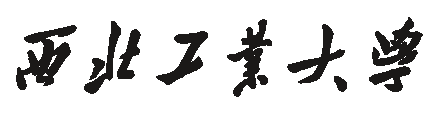
\includegraphics[width=10.48cm,height=1.69cm]{pic/university_text_logo}\\
		\vspace{9pt}
		\sXiaoyi \fSong \bfseries{研究生课程考试答题册}
	\end{center}
	
	% 连续三个四号的空格 14.4*3
	% \vspace{43.2pt}
	\sSihao ~ \\
	
	
	% 得分表
	% 宽4.3 高1.92
	
	
	\begin{table}[h]
		%	\renewcommand\arraystretch{2}
		\begin{tabular}[c]{m{8cm}|m{4.32cm}|c}
			\cline{2-2}
			& \vspace{.8cm} \sSihao \fKai 得分: \vspace{.8cm} & \\
			\cline{2-2}
			
		\end{tabular}
	\end{table}
	
	% 小四空格
	% \vspace{14.4pt}
	\sSihao ~\\
	
	% 填空
	\begin{center}
		%\vskip 2cm
		{
			\fKai \sSihao 学~~~~~~~~号 \coverunderline[8cm]{}\\
			%\vskip 0.7cm
			\fKai \sSihao 姓~~~~~~~~名 \coverunderline[8cm]{}\\
			%\vskip 0.7cm
			\fKai \sSihao 考试课程 \coverunderline[8cm]{几何造型原理和应用}\\
			%\vskip 0.7cm
			\fKai \sSihao 考试时间 \coverunderline[8cm]{2017年12月30日}
			%\vfill
		}
	\end{center}
\end{titlepage}